\section{Clinical Integration and Workflow}
\label{sec:clinical-integration}

The integration of the Robotic Ultrasound System (RUS) into clinical environments requires careful consideration of medical workflows, regulatory compliance, and user experience design. This section examines the clinical deployment aspects of the system.

\subsection{Clinical Workflow Integration}

\subsubsection{Pre-Procedure Setup}
The system's clinical workflow begins with automated setup procedures that minimize manual configuration:

\begin{lstlisting}[language=C++, caption={Clinical Setup Protocol}, label={lst:clinical-setup}]
class ClinicalWorkflowManager {
private:
    SystemCalibration calibration_;
    PatientSafetyMonitor safety_monitor_;
    QualityAssuranceModule qa_module_;
    
public:
    bool initializeClinicalSession(const PatientData& patient) {
        // Verify system calibration
        if (!calibration_.verifyCalibration()) {
            LOG_ERROR("System calibration verification failed");
            return false;
        }
        
        // Initialize safety monitoring
        safety_monitor_.configureForPatient(patient);
        
        // Run quality assurance checks
        return qa_module_.performPreProcedureChecks();
    }
    
    void configureForProcedureType(ProcedureType type) {
        switch(type) {
            case DIAGNOSTIC_SCAN:
                configureForDiagnostic();
                break;
            case GUIDED_INTERVENTION:
                configureForIntervention();
                break;
            case FOLLOW_UP_ASSESSMENT:
                configureForFollowUp();
                break;
        }
    }
};
\end{lstlisting}

\subsubsection{Intra-Procedure Monitoring}
During active procedures, the system provides real-time monitoring and adaptive control:

\begin{figure}[htbp]
\centering
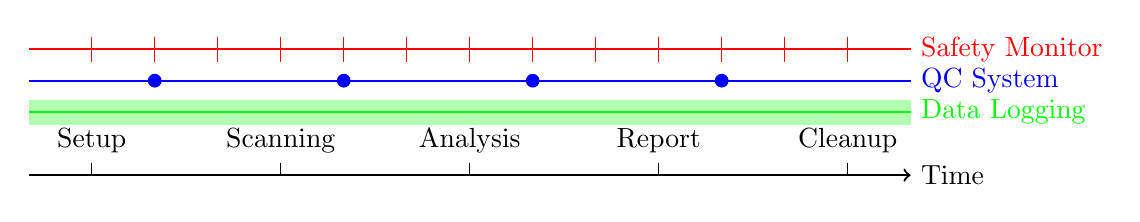
\begin{tikzpicture}[scale=0.8]
    % Clinical workflow timeline
    \draw[thick, ->] (0,0) -- (14,0) node[right] {Time};
    
    % Workflow phases
    \foreach \x/\label in {1/Setup, 4/Scanning, 7/Analysis, 10/Report, 13/Cleanup} {
        \draw (\x,0) -- (\x,0.2);
        \node[above] at (\x,0.2) {\label};
    }
    
    % Safety monitoring
    \draw[red, thick] (0,2) -- (14,2) node[right] {Safety Monitor};
    \foreach \x in {1,2,3,...,13} {
        \draw[red] (\x,1.8) -- (\x,2.2);
    }
    
    % Quality control
    \draw[blue, thick] (0,1.5) -- (14,1.5) node[right] {QC System};
    \foreach \x in {2,5,8,11} {
        \draw[blue, fill=blue] (\x,1.5) circle (0.1);
    }
    
    % Data logging
    \draw[green, thick] (0,1) -- (14,1) node[right] {Data Logging};
    \fill[green, opacity=0.3] (0,0.8) rectangle (14,1.2);
    
\end{tikzpicture}
\caption{Clinical Workflow Timeline with Integrated Monitoring Systems}
\label{fig:clinical-workflow}
\end{figure}

\subsection{User Interface Design for Clinical Environments}

\subsubsection{Clinician-Centric Interface}
The system interface is designed with clinical usability principles:

\begin{itemize}
    \item \textbf{Minimal Cognitive Load}: Intuitive controls with clear visual feedback
    \item \textbf{Error Prevention}: Confirmations for critical actions
    \item \textbf{Rapid Access}: One-touch access to emergency stops and critical functions
    \item \textbf{Sterile Operation}: Touch-free controls and voice commands where applicable
\end{itemize}

\begin{table}[htbp]
\centering
\caption{Interface Usability Requirements}
\label{tab:usability-requirements}
\begin{tabular}{|l|l|l|}
\hline
\textbf{Requirement} & \textbf{Specification} & \textbf{Validation Method} \\
\hline
Response Time & $< 100$ ms for critical actions & Automated testing \\
Error Rate & $< 0.1\%$ for routine operations & Clinical trials \\
Learning Curve & $< 2$ hours for basic proficiency & User studies \\
Accessibility & WCAG 2.1 AA compliance & Accessibility audit \\
\hline
\end{tabular}
\end{table}

\subsubsection{Multi-Modal Interaction}
The system supports various interaction modalities to accommodate different clinical scenarios:

\begin{lstlisting}[language=C++, caption={Multi-Modal Interface Handler}, label={lst:multimodal-interface}]
class ClinicalInterface {
private:
    TouchController touch_interface_;
    VoiceRecognition voice_commands_;
    GestureRecognition gesture_control_;
    EyeTracking gaze_interface_;
    
public:
    void processUserInput() {
        // Priority-based input handling
        if (voice_commands_.hasEmergencyCommand()) {
            handleEmergencyCommand();
            return;
        }
        
        if (touch_interface_.hasCriticalInput()) {
            handleTouchInput();
            return;
        }
        
        // Normal operation input processing
        processRoutineInputs();
    }
    
    void adaptToSterileEnvironment(bool sterile_mode) {
        if (sterile_mode) {
            touch_interface_.disable();
            voice_commands_.setSensitivity(HIGH);
            gesture_control_.enable();
        } else {
            enableAllInteractionModes();
        }
    }
};
\end{lstlisting}

\subsection{Patient Safety Systems}

\subsubsection{Real-Time Safety Monitoring}
The system implements multiple layers of patient safety monitoring:

\begin{figure}[htbp]
\centering
\begin{tikzpicture}[scale=0.9]
    % Safety monitoring architecture
    \node[draw, rectangle, fill=red!20] (sensor) at (0,0) {Sensor Layer};
    \node[draw, rectangle, fill=orange!20] (detect) at (3,0) {Detection Layer};
    \node[draw, rectangle, fill=yellow!20] (analyze) at (6,0) {Analysis Layer};
    \node[draw, rectangle, fill=green!20] (response) at (9,0) {Response Layer};
    
    % Connections
    \draw[->] (sensor) -- (detect);
    \draw[->] (detect) -- (analyze);
    \draw[->] (analyze) -- (response);
    
    % Safety components
    \node[below=0.5cm of sensor] {Force Sensors};
    \node[below=1cm of sensor] {Position Monitors};
    \node[below=1.5cm of sensor] {Pressure Sensors};
    
    \node[below=0.5cm of detect] {Anomaly Detection};
    \node[below=1cm of detect] {Pattern Recognition};
    \node[below=1.5cm of detect] {Threshold Monitoring};
    
    \node[below=0.5cm of analyze] {Risk Assessment};
    \node[below=1cm of analyze] {Trend Analysis};
    \node[below=1.5cm of analyze] {Predictive Modeling};
    
    \node[below=0.5cm of response] {Emergency Stop};
    \node[below=1cm of response] {Gradual Adjustment};
    \node[below=1.5cm of response] {Alert Generation};
    
\end{tikzpicture}
\caption{Multi-Layer Patient Safety Monitoring Architecture}
\label{fig:safety-monitoring}
\end{figure}

\subsubsection{Emergency Response Protocols}
The system implements standardized emergency response procedures:

\begin{lstlisting}[language=C++, caption={Emergency Response System}, label={lst:emergency-response}]
class EmergencyResponseSystem {
private:
    enum EmergencyLevel {
        LOW_PRIORITY,
        MEDIUM_PRIORITY,
        HIGH_PRIORITY,
        CRITICAL
    };
    
    std::map<EmergencyLevel, std::chrono::milliseconds> response_times_ = {
        {CRITICAL, std::chrono::milliseconds(10)},
        {HIGH_PRIORITY, std::chrono::milliseconds(50)},
        {MEDIUM_PRIORITY, std::chrono::milliseconds(200)},
        {LOW_PRIORITY, std::chrono::milliseconds(1000)}
    };
    
public:
    void handleEmergency(EmergencyLevel level, const std::string& reason) {
        auto start_time = std::chrono::high_resolution_clock::now();
        
        switch(level) {
            case CRITICAL:
                executeImmediateStop();
                alertMedicalStaff();
                logCriticalEvent(reason);
                break;
                
            case HIGH_PRIORITY:
                pauseCurrentOperation();
                assessSituation();
                requestUserConfirmation();
                break;
                
            case MEDIUM_PRIORITY:
                adjustOperationParameters();
                notifyOperator();
                break;
                
            case LOW_PRIORITY:
                logWarning(reason);
                displayStatusMessage();
                break;
        }
        
        auto response_time = std::chrono::high_resolution_clock::now() - start_time;
        validateResponseTime(level, response_time);
    }
};
\end{lstlisting}

\subsection{Data Management and Privacy}

\subsubsection{HIPAA Compliance}
The system ensures comprehensive protection of patient health information:

\begin{itemize}
    \item \textbf{Encryption}: AES-256 encryption for data at rest and in transit
    \item \textbf{Access Control}: Role-based access with multi-factor authentication
    \item \textbf{Audit Trails}: Complete logging of all data access and modifications
    \item \textbf{Data Minimization}: Collection and retention of only necessary data
\end{itemize}

\begin{table}[htbp]
\centering
\caption{HIPAA Compliance Implementation}
\label{tab:hipaa-compliance}
\begin{tabular}{|l|l|l|}
\hline
\textbf{HIPAA Requirement} & \textbf{Implementation} & \textbf{Validation} \\
\hline
Access Control & RBAC with MFA & Penetration testing \\
Audit Logging & Complete activity logs & Log analysis tools \\
Data Encryption & AES-256 & Cryptographic validation \\
Backup Security & Encrypted backups & Recovery testing \\
Physical Safeguards & Secure hardware & Security assessment \\
\hline
\end{tabular}
\end{table}

\subsubsection{Clinical Data Integration}
The system integrates with existing hospital information systems:

\begin{lstlisting}[language=C++, caption={Clinical Data Integration}, label={lst:clinical-data}]
class ClinicalDataIntegrator {
private:
    HISConnector his_connector_;
    PACSInterface pacs_interface_;
    EMRIntegration emr_integration_;
    
public:
    bool integrateWithHospitalSystems() {
        // Establish secure connections
        if (!his_connector_.establishSecureConnection()) {
            LOG_ERROR("Failed to connect to HIS");
            return false;
        }
        
        // Configure PACS integration
        pacs_interface_.configureDICOMSettings();
        
        // Setup EMR data exchange
        return emr_integration_.initializeHL7Interface();
    }
    
    void exportScanResults(const ScanData& scan_data) {
        // Generate DICOM-compliant images
        auto dicom_images = generateDICOMImages(scan_data);
        
        // Upload to PACS
        pacs_interface_.uploadImages(dicom_images);
        
        // Update EMR with scan results
        emr_integration_.updatePatientRecord(scan_data.getPatientID(), 
                                           scan_data.getResults());
        
        // Archive data according to retention policy
        archiveManager_.scheduleArchival(scan_data);
    }
};
\end{lstlisting}

\subsection{Training and Certification}

\subsubsection{Operator Training Program}
The system includes a comprehensive training program for clinical operators:

\begin{enumerate}
    \item \textbf{Basic Operation}: System startup, calibration, and routine procedures
    \item \textbf{Safety Protocols}: Emergency procedures and patient safety measures
    \item \textbf{Quality Assurance}: Image quality assessment and troubleshooting
    \item \textbf{Maintenance}: Routine maintenance and basic diagnostics
\end{enumerate}

\begin{figure}[htbp]
\centering
\begin{tikzpicture}[scale=0.8]
    % Training progression
    \node[draw, circle, fill=blue!20, align=center] (basic) at (0,0) {Basic\\Training};
    \node[draw, circle, fill=green!20, align=center] (intermediate) at (4,0) {Intermediate\\Skills};
    \node[draw, circle, fill=orange!20, align=center] (advanced) at (8,0) {Advanced\\Operation};
    \node[draw, circle, fill=red!20, align=center] (expert) at (12,0) {Expert\\Certification};
    
    % Progression arrows
    \draw[->] (basic) -- (intermediate);
    \draw[->] (intermediate) -- (advanced);
    \draw[->] (advanced) -- (expert);
    
    % Training duration
    \node[below=1cm of basic] {2 days};
    \node[below=1cm of intermediate] {1 week};
    \node[below=1cm of advanced] {2 weeks};
    \node[below=1cm of expert] {1 month};
    
    % Competency requirements
    \node[above=1cm of basic] {Basic Operation};
    \node[above=1cm of intermediate] {Safety Protocols};
    \node[above=1cm of advanced] {Quality Control};
    \node[above=1cm of expert] {System Optimization};
    
\end{tikzpicture}
\caption{Clinical Training Progression Pathway}
\label{fig:training-progression}
\end{figure}

\subsubsection{Continuous Education and Updates}
The system supports ongoing professional development:

\begin{itemize}
    \item \textbf{Regular Updates}: Automatic delivery of new features and protocols
    \item \textbf{Performance Monitoring}: Tracking of operator competency and outcomes
    \item \textbf{Continuing Education}: Integration with medical education platforms
    \item \textbf{Peer Learning}: Collaboration tools for knowledge sharing
\end{itemize}

This clinical integration framework ensures that the RUS system can be effectively deployed in healthcare environments while maintaining the highest standards of patient safety, data security, and operational efficiency.
